\section{Architektur}
Das Projekt besteht aus einer ausführbaren Applikation (app\textunderscore basic), welche grundsätzlich nur alle \glspl{Plugin} lädt.
Die Plugins bilden die eigentlich wichtigen Teile der Applikation, sie beinhalten die Übungen und Lösungen.
Jedes Plugin ist eine in sich abgeschlossene Anwendung, welche für einen spezifischen Use-Case erstellt wurde, z.B.
das Fliegen der Drohne mithilfe der Tastatur oder das Fliegen der Drohne über Objekterkennung.
\begin{figure}[H]
    \centering
    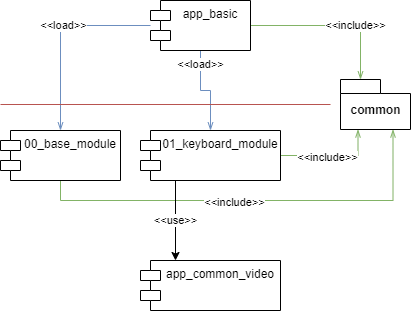
\includegraphics[width=0.6\textwidth]{../common/chapter_01/resources/02_architecture.png}
    \captionof{figure}{Architektur}
\end{figure}
Wenn du in einem der Module (Plugin) Änderungen gemacht hast, dann musst du dieses Modul neu kompilieren. Wähle
dazu dieses Modul als Startlement in Visual Studio 2019 oder als 'target' in CLion aus und führe die Kompilierung
durch. Wenn du anschliessend die Hauptapplikation startest, wirst du deine Änderungen sehen.
Wenn du bei einer Aufgabe nicht weiter wissen solltest, kannst du einen Blick in die Referenzimplementation werfen.
Diese enden mit der Bezeichnung '\textunderscore solution'. Jeder Übungsabschnitt beinhaltet die entsprechenden
Lösungen am Ende des Kapitels.
Und nun, viel Spass bei den Übungen.